\section{Sprint 5}
Im fünften Sprint wurde zwei weiter Zusatzfeatures eingeplant, welche von den Nutzern gewünscht wurden.
Eine weitere Story befasst sich mit einer kleinen Verbesserung des Object Models.
Dies sind die Stories:
\begin{itemize}
   \item Implementation einer Suchfunktion für das Object Model
   \item Implementation einer Filterfunktion für das Object Model
   \item Das Lesen und Schrieben von Enum Werten soll verbessert werden.
\end{itemize}

\subsection{Suchfunktion}
\dq Implementation einer Suchfunktion für das Object Model\dq
\subsubsection{Ziel}
Die Object Models bestehe aus mehreren hundert Objekten und tausenden Attributen und Methoden.
Eine Suchfunktion soll das finden eines spezifischen Objekts oder einer Gruppe von Objekten erleichtern.
Ebenfalls soll es mögliche sein, bestimmte Attribute oder Methoden zu finden, ohne die dazugehörige Klasse zu kennen.
Bei der Suche soll nach Name, Titel und Obis Code der Objekte gesucht werden.
Für Attribute und Methode soll jeweils nur der Name verwendet werden.
Die Gross- und Kleinschreibung soll dabei ignoriert werden.
Dass ein Element in den Suchergebnissen erscheint muss der Suchbegriff vollständig enthalten sein.

\subsubsection{Vorgehen und Schwierigkeiten}
Im Abschnitt \ref{searchandfilterUiSktech} wird ein Konzept für die Darstellung der Such- und Filterkomponente erklärt.
Für diese Story wurde die Benutzerschnittstelle für die Suche nach diesem Konzept umgesetzt.
Der geplante Platz für die Filterkomponente wurde frei gelassen, da diese in der Folgestory implementiert wird.
In Klassendiagramm \ref{fig:objectModelVMClassDiagram} ist das Interface \textit{IObjectModelViewModel} abgebildet.
\begin{figure}
   \centering
   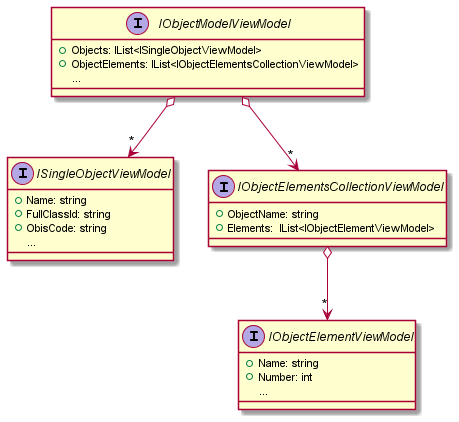
\includegraphics[width=0.7\textwidth]{gfx/OMVM.png}
   \caption{
      Reduziertes Klassendiagramm zu IObjectModelViewModel
      }
      \label{fig:objectModelVMClassDiagram}
\end{figure}
Über diese werden alle Daten abgerufen, welche für die Darstellung der Object Model Komponente benötigt werden.
Die Liste \textit{Objects} beinhaltete alle Objekte, welche im Object Model angezeigt werden.
Die Suchfunktion wie folgt implementieren:
\begin{enumerate}
   \item Die Suche wird mit einem Klick auf den \textit{Find} Knopf gestartet.
   \item Alle \textit{ISingleObjectViewModel} Objekte werden aus der \textit{Objects} Liste entfernt.
   \item Die \ac{COSEM} Objekte werden anhand des Suchtexts gefiltert.
   \item Für jedes verbleibende Objekt wird eine neues \textit{ISingleObjectViewModel} erstellt und der \textit{Objects} Liste hinzugefügt.
\end{enumerate} 
Diese Implementation war funktional ausreichend, war jedoch teilweise sehr langsam.
Je mehr Objekte als Suchresultat dargestellt werden mussten, desto langsamer wurde die Suche.
Dies hatte damit zu tun, dass für jedes Objekt ein neues \textit{ISingleObjectViewModel} Objekt erstellt wurde.
Um dies zu verbessern wurde ein Cache eingesetzt, welcher anstelle eines neuen Objekt jeweils ein bestehendes liefert.

Um nicht nach Objekten sondern nach Attributen und Methoden zu suchen, wurde etwas ähnliches implementiert.
Im Klassendiagramm ist das Interface \textit{IObjectElementsCollectionViewModel} aufgezeigt.
Dieses fasst alle Attribute und Methoden einer Klasse zusammen, welche dargestellt werden sollen.
Im Property \textit{ObjectElements} wird eine Liste dieser Objekte gehalten.
Diese wird mit dem gleichen Vorgehen wie bei den Objekten auf jenen Elemente reduziert, welche den Suchkriterien entsprechen.
In Abbildung \ref{fig:searchforClock} ist die Suche nach Attributen und Methoden dargestellt.


\begin{figure}
   \centering
   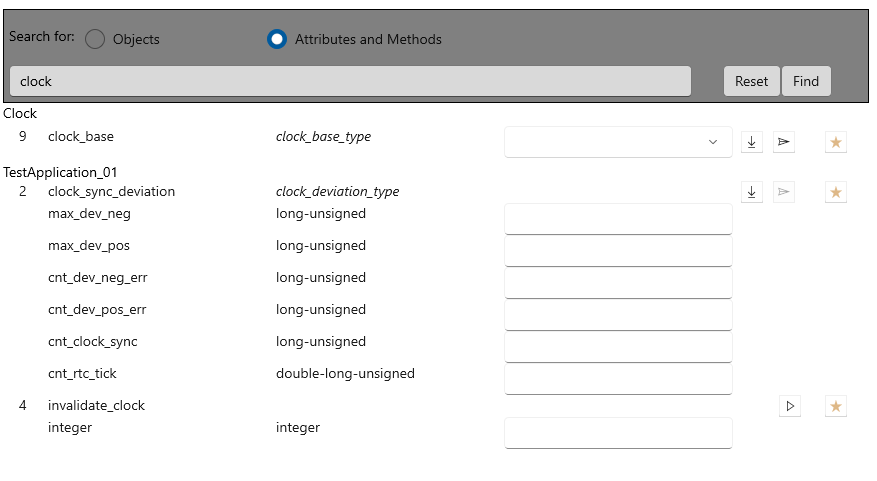
\includegraphics[width=1.0\textwidth]{gfx/searchforclick.png}
   \caption{
      Resultate der Suche nach Attributen und Methoden mit dem Text \dq clock\dq
      }
      \label{fig:searchforClock}
\end{figure}




\subsection{Filterfunktion}
\dq Implementation einer Filterfunktion für das Object Model\dq
\subsubsection{Ziel}
Um Objekte einer bestimmten \ac{COSEM} Klasse anzuzeigen, soll eine Filterfunktion implementiert werden.
Es soll möglich sein, dass nach Class Id, Class Version, Own Class Version und Sub Type gefiltert werden können.
\subsubsection{Vorgehen und Schwierigkeiten}
\begin{figure}
   \centering
   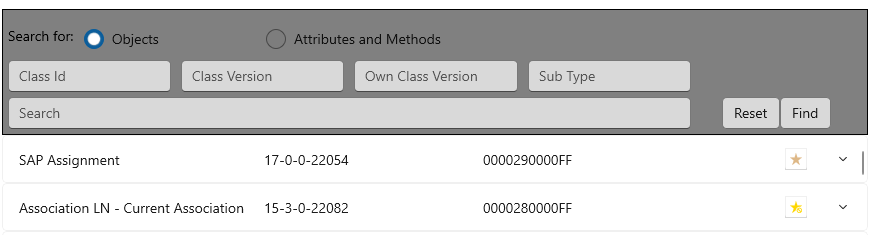
\includegraphics[width=1.0\textwidth]{gfx/searchfilter.png}
   \caption{
      Such- und Filterfunktion aus DlmsQuickAccess 
      }
      \label{fig:searchfilterUIRel}
\end{figure}
Die Filterfunktion wurde bereits bei den Arbeiten an der Suchfunktion berücksichtigt.
In der Benutzerschnittstelle wurden die zusätzlichen Textfelder hinzugefügt.
Abbildung \ref{fig:searchfilterUIRel} zeigt diese.
Der Algorithmus, welcher die \ac{COSEM} Objekte bisher nach Suchtext filtert wurde so erweitert, dass die neu hinzugefügten Parameter berücksichtigt werden.
Dies konnte ohne Schwierigkeiten umgesetzt werden.



\subsection{Enums}
\dq Das Lesen und Schrieben von Enum Werten soll verbessert werden.\dq
\subsubsection{Ziel}
Im \ac{DMT2} sowie in den bisherigen Versionen des DlmsQuickAccess wurden Enums gleich wie andere Zahlenwerte behandelt.
Nutzer der Anwendungen mussten jeweils die Class Description der entsprechenden Klasse abrufen, um die Bedeutung eines bestimmten Werts zu erfahren.
Dies soll verbessert werden, indem anstelle des Nummer die dazugehörige Bezeichnung angezeigt wird.

\subsubsection{Vorgehen und Schwierigkeiten}
Im Text zur Realisierung des zweiten Sprints (\ref{readAttributVorgehen}) wurde erklärt, dass für die optimale Darstellung des Object Models Informationen aus der XML Datei es Object Models um jene der Class Descriptions erweitert wurden.
Zu diesen Informationen gehören auch die Bezeichnungen der Enums.
In Abbildung \ref{fig:enumTypedefword} ist ein Ausschnitt aus einer Class Description gezeigt, welcher die Definition eines Enum-Types beinhaltet.
\begin{figure}
   \centering
   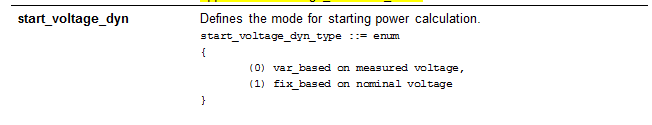
\includegraphics[width=1.0\textwidth]{gfx/enum_typedef_word.png}
   \caption{
      Ausschnitt aus dem Word Dokument einer Class Description
      }
      \label{fig:enumTypedefword}
\end{figure}
In der XML Repräsentation der Class Description, welche vom DlmsQuickAccess eingelesen wird, sieht diese Typendefinition wie folgt aus:
\begin{verbatim}
<cm:typedefinition name="start_voltage_dyn_type" base="enum">
   <cm:item name="var_based on measured voltage" value="0" />
   <cm:item name="fix_based on nominal voltage" value="1" />
</cm:typedefinition>
\end{verbatim}

Im Abschnitt \ref{readAttributVorgehen} wurde erklärt, dass das Adapter Pattern verwendet wurde, um die Class Descriptions in die gewünschte Klassenstruktur zu überführen.
Als versucht wurde, auf die einzelnen Enum Werte zuzugreifen, traten Fehler bei der Implementation der Adapter auf.
Diese zeigten sich dann, wenn mehrere Typendefinitionen ineinander verschachtelt sind.
Dies kommt beispielsweise vor, wenn es sich beim Typen eines Attributes um ein Array handelt, wessen Elemente jeweils Strukturen sind, welche ein Feld von Type Enum enthalten.
Bei Lösen diesen Fehler zeigte sich durch eine erschwerte Testbarkeit, dass das Adapter Pattern nicht optimal angewendet wurde.
Deshalb wurden einige Klassen grundlegend überarbeitet.

Rückblickend musst kann gesagt werden, dass das Verwenden des Codes der \textit{InfraLib} nicht zu den erhofften Zeitersparnissen geführt hat.
Die Library war nicht ausreichend getestet und einige erwarteten Funktionen fehlten ganz.
Eine von Grund auf eigene Implementation für das Parsing der Class Description wäre vermutlich mit weniger Zeitaufwand verbunden gewesen und hätte zu einer besseren Lösung geführt.

% - Repo aufräumen
% Probleme mit "ObjectModel" oder "Attribute" namespace
